\section{Durchführung}
\label{sec:Durchführung}
Der schematische Aufbau der Messapparatur ist in \autoref{fig:aufbau} dargestellt.

\begin{figure}
    \centering
    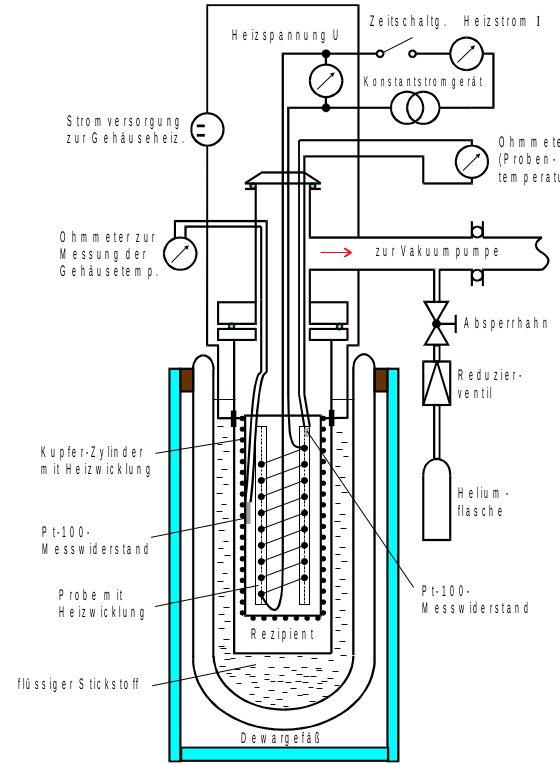
\includegraphics[width=0.8\linewidth]{abb/aufbau.png}
    \caption{Schematischer Aufbau der Messapparatur \cite{sample}.}
    \label{fig:aufbau}
\end{figure}

Zu Beginn wird der Rezipient evakuiert und anschließend bei Barometerdruck mit Helium gefüllt.
Daraufhin wird das Dewargefäß, in dem sich der Rezipient befindet, mit flüssigem Stickstoff gefüllt um die Kupferprobe auf \qty{80}{\kelvin} abzukühlen.
Obwohl Helium ein schlechterer Wärmeleiter als Luft ist, kommt es hier zum Einsatz um eine Verunreinigung durch frierendes Wasser im Rezipienten zu verhindern.
Nach erreichen der gewünschten Temperatur wird jedoch wieder die Vakuumpumpe eingeschaltet, bis die Pumpleistung gleich der Leckrate ist und
ein möglichst niedriger gleichbleibender Druck herrscht. Dies ist neben der Notwendigkeit zur Messung von $C_p$ auch von Nutzen um Wärmekonvektion zu verhindern.
Während der Messung wird der Probe durch eine Heizwicklung einer Gleichstromquelle Wärme zugeführt.
Um weitere unvorteilhafte Abgänge der eingegangenen Heizleistung zu verhindern wird ein Kupferzylinder, der die Probe umschließt, gleichermaßen durch eine
zweite Gleichstromquelle erhitzt um potentieller Wärmestrahlung entgegenzuwirken.
Der dritte mögliche Verlust, die Wärmeleitung, wird durch eine möglichst geringe Fläche seitens der Aufhängung im Rezipienten minimiert.

Gemessen werden die Temperaturen $T$ der Probe sowie des Zylinders, die Heizspannung $U$ und der Heizstrom $I$ der Proben-Heizwicklung und die abgelaufene Zeit $t$.
Die Messung gilt als abgeschlossen, falls eine Probentemperatur von etwa \qty{300}{\kelvin} erreicht wurde.
Möglichst sollten die Temperaturabstände gleichmäßig \qty{10}{\kelvin} betragen. Die Temperatur wird jeweils durch eine Messung
über ein digitales Ohmmeter eines Pt-100 Widerstandes $R$ aufgenommen. Dessen Temperaturzusammenhang lautet:
\begin{equation}
    \label{eq:Temp}
    T = 0.00134 R^2 + 2.296 R - 243.02 \; .
\end{equation}